\documentclass[lang=cn,10pt]{elegantbook}
\usepackage{physics}
\usepackage {circuitikz}
\usepackage{ulem}%下划线
\usepackage{hyperref}%目录跳转



\title{HappaMathsNotes}
\subtitle{解析几何}
\author{OyamaHappa}
\bioinfo{数学}{学无止境}
\extrainfo{数学是人类智慧皇冠上最灿烂的明珠。——考特}
\date{\today}
\version{20240719105707}
\logo{logo.jpg}
\cover{cover.jpg}



% 本文档命令
\usepackage{array}
\usepackage{mathdots}
\newcommand{\ccr}[1]{\makecell{{\color{#1}\rule{1cm}{1cm}}}}
% 修改目录深度
\setcounter{tocdepth}{3}

\everymath{\displaystyle}%用行间公式(displaystyle)的格式排版所有的行内公式


%\usepackage{verbatim}%在codeshow中已引用
\usepackage{tikz,tkz-euclide}
\usepackage{amsmath}
\usepackage{pgfplots}
%\usepackage{codeshow}%codeshow:为了在codeshow环境中,引用代码,并生成图形。

\usepackage{graphicx}
%\usepackage{subfigure}

\usepackage{breqn}%breqn 宏包主要提供了 dmath 和 dmath* 等几个环境,产生可以自动折行的显示公式。
\usepackage{longtable}%长表格,多页可以自动处理。

%【参与编译的文件列表。】
%\includeonly{preface,chapter01,chapter02,chapter03,chapter04,chapter05}%,%【参与编译的文件列表。】
\usepackage{longtable}%长表格
\usepackage{amsmath}
\usepackage{tcolorbox}%


\usepackage{pgfplots} % 导入pgfplots包以绘制图形
\usepackage{amsmath} % 导入amsmath包以使用高级数学公式


\begin{document}
	\maketitle
	
	\tableofcontents
	%\listofchanges
	
	\mainmatter
\chapter{解析几何}

	\section{直线的方程}
	
	\[ Ax+By+C=0 \Longrightarrow y=-\dfrac{A}{B}-\dfrac{C}{B}\]
	
	$l_{1}$ $ \parallel$ $ l_{2}$ $\Longrightarrow$ $k_{1} = k_{2}$ $ \Longrightarrow$ $ A_{1}\textperiodcentered B_{2}=A_{2}\textperiodcentered B_{1} \mbox{且} B_{1} \textperiodcentered C_{2} \neq B_{2}\textperiodcentered C_{1}$
	
	$l_{1}$ $ \perp$ $ l_{2}$ $\Longrightarrow$ $k_{1} \textperiodcentered k_{2} =-1$ $\Rightarrow$ $A_{1}\textperiodcentered A_{2}+B_{1}\textperiodcentered B_{2}=0$
	
	方向向量(B,-A)
	法向量(A,B)
	
	$cos\theta = \dfrac{1}{\sqrt{1+k^{2}}} = \dfrac{1}{\sqrt{1+\dfrac{A^{2}}{B^{2}}}} = \dfrac{|B|}{\sqrt{A^{2}+B^{2}}}$
	\subsection{点到直线距离公式}
	\[d=\dfrac{|Ax_{0}+By_{0}+C|}{\sqrt{A^{2}+B^{2}}}\]
	\subsection{直线到直线距离公式}
	$d=\varDelta y \textperiodcentered cos\theta = |-\dfrac{C_{1}}{B}+\dfrac{C_{2}}{B}| \textperiodcentered \dfrac{B}{\sqrt{A^{2}+B^{2}}} =\dfrac{|C_{2}-C_{1}|}{\sqrt{A^{2}+B^{2}}}$
	\[d=\dfrac{|C_{2}-C_{1}|}{\sqrt{A^{2}+B^{2}}}\]
	
	\subsection{对称}
	\subsubsection{点关于点对}
	$ A(x_{1},y_{1})$ 关于 $P(x_{0},y_{0})$ 对称点$(2x_{0}-x_{1},2y_{0}-y_{1})$
		\subsubsection{点关于线对称}
	$A\dfrac{x_{1}+x_{2}}{2}+B{y_{1}+y_{2}}{2}+C=0$\\
	$-\dfrac{A}{B} \textperiodcentered \dfrac{y^{2}-y^{1}}{x_{2}=x_{1}}=-1$
			\subsubsection{线关于点对称}
			\subsubsection{线关于线对称}
	\paragraph{平行}~{}\\
	\[C_{2}-C_{1}=C_{3}-C_{2}\]
	\paragraph{不平行}~{}\\
	$tan(\theta_{1} -\theta_{2})$ = $tan(\theta_{2} -\theta_{3})\Rightarrow$ $\dfrac{k_{1}-k_{2}}{1+k_{1}k_{2}}=\dfrac{k_{2}-k_{3}}{1+k_{2}k_{3}}$\\
	\[\dfrac{k_{1}-k_{2}}{1+k_{1}k_{2}}=\dfrac{k_{2}-k_{3}}{1+k_{2}k_{3}}\]
	\[\mbox{\textbf{到角公式}}\]
	
	\section{圆的方程}
	$ x^{2}+y^{2}+Dx+Ey+F=0\Rightarrow(x+\dfrac{D}{2})^{2}+(y+\dfrac{E}{2})^{2}=\dfrac{D^{2}+E^{2}+4F}{4}>0$
	\subsection{圆的直径式方程}~{}\\    
	\[(x-a)(x-c)+(y-b)(y-d)=0\]
	\subsection{阿波罗尼斯圆}~{}\\  
	动点到两定点的距离之比为定值(k $\neq$ 1)  则动点轨迹为圆
	\subsection{圆的参数方程}~{}\\
	$
	\left\{
	\begin{aligned}
		x = & \cos(\theta) \\
		y = & \sin(\theta) \\
	\end{aligned}
	\right.
	$
	\subsubsection{三角换元}~{}\\
	\[(x-a)^{2}+(y-b)^{2}=R^{2}\]
	$
	\left.
	\begin{aligned}
		x - a = & \cos(\theta) \\
		y -b = & \sin(\theta) \\
	\end{aligned}
	\right\}
	\Rightarrow
	\left\{
	\begin{aligned}
		x = & a+R\textperiodcentered \cos(\theta) \\
		y = & b+ R\textperiodcentered\sin(\theta) \\
	\end{aligned}
	\right.
	$
	
	
	\subsection{直线与圆位置关系}~{}\\
	\[d=\dfrac{|Aa+Bb+C|}{\sqrt{A^{2}+B^{2}}}\]
	\subsubsection{直线与圆相离}~{}\\ 
	\[d_{min}=d-r\]
	\[d_{MAX}=d+r\]
	\paragraph{$d'\Rightarrow$要求距离}~{}\\ 
	$d=r+d' \Rightarrow 1 \mbox{个} $\\
	$r-d'<d<r+d'\Rightarrow 2 \mbox{个}$\\
	$d=r-d''\Rightarrow 3 \mbox{个}$\\
	$0\leq d<r-d' \Rightarrow 4 \mbox{个}$\\
	
	$O_{1}O_{2}>r_{1}+r_{2} \Rightarrow$相离,4条公切线\quad $O_{1}O_{2}=r_{1}+r_{2} \Rightarrow$外切,3条公切线\\
	 $|r_{1}-r_{2}|<O_{1}O_{2}<r_{1}+r_{2} \Rightarrow$相交,2条公切线\quad $O_{1}O_{2}=|r_{1}-r_{2}| \Rightarrow$内切,1条公切线\\
     $0<O_{1}O_{2}<|r_{1}-r_{2}| \Rightarrow$内含,0条公切线\quad  $O_{1}O_{2}=0 \Rightarrow$同心圆,0条公切线\quad
     	\subsection{圆系方程}~{}\\
     	\[ \lambda(Ax+By+C)+x^{2}+y^{2}+Dx+Ey+F=0\]
\[
\left\{
\begin{aligned}
	Ax + By + C &= 0 \\
	x^2 + y^2 + Dx + Ey + F &= 0
\end{aligned}
\right\}
\Rightarrow \text{交点}
\]
	\[\]
	\[\]
		\[ \lambda(x^{2}+y^{2}+D_{1}x+E_{1}y+F_{1})+x^{2}+y^{2}+D_{2}x+E_{2}y+F_{2}=0\]
		\[
		\left\{
		\begin{aligned}
			x^{2}+y^{2}+D_{1}x+E_{1}y+F_{1} &= 0 \\
			x^{2}+y^{2}+D_{2}x+E_{2}y+F_{2} &= 0
		\end{aligned}
		\right\}
		\Rightarrow \text{定点}\Leftrightarrow \mbox{交点}
		\]
	\[ \star x=-1\]
	\subsubsection{$\Rightarrow$公共弦}
			$
	\left\{
	\begin{aligned}
		x^{2}+y^{2}+D_{1}x+E_{1}y+F_{1} &= 0 \\
		x^{2}+y^{2}+D_{2}x+E_{2}y+F_{2} &= 0
	\end{aligned}
	\right\}
	\Rightarrow l_{1}:(D_{1}=D_{2})x+(E_{1}-E_{2})y+(F_{1}-F_{2})=0
	$
	\[l_{1}:(D_{1}=D_{2})x+(E_{1}-E_{2})y+(F_{1}-F_{2})=0\]
\section{椭圆}
\subsection{第一定义}
动点到两定点和为定值\ 即动点轨迹为椭圆\\

\begin{tikzpicture}
	% 绘制椭圆,中心在 (0,0),长轴长为 8,短轴长为 4
	\draw[thick] (0,0) ellipse (4 and 2);
	
	% 绘制长轴(虚线),从 (-4,0) 到 (4,0)
	\draw[dashed] (-4,0) -- (4,0);
	% 绘制短轴(虚线),从 (0,-2) 到 (0,2)
	\draw[dashed] (0,-2) -- (0,2);
	
	% 标注长轴,在 (4.5,0) 处添加文字“长轴”
	\node at (2,0.25) {长轴2a};
	% 标注短轴,在 (0,2.5) 处添加文字“短轴”
	\node at (1,1) {短轴2b};
	
	% 计算焦点的位置
	\pgfmathsetmacro{\a}{4} % 半长轴长度
	\pgfmathsetmacro{\b}{2} % 半短轴长度
	\pgfmathsetmacro{\c}{sqrt(\a*\a - \b*\b)} % 焦点距中心的距离,公式 c = sqrt(a^2 - b^2)
	
	% 绘制焦点 F1,在 (\c, 0) 处画一个半径为 2pt 的实心圆,并标注 F1
	\fill ( \c, 0) circle (2pt) node[above] {$F_1$};
	% 绘制焦点 F2,在 (-\c, 0) 处画一个半径为 2pt 的实心圆,并标注 F2
	\fill (-\c, 0) circle (2pt) node[above] {$F_2$};
	
	% 标注中心点,在 (0,0) 处添加文字“O”
	\node[below right] at (0,0) {O};

 % 绘制通过焦点的直线(通经)
\draw[dotted] (\c,2.5) -- (\c,-2.5); % x = +c
\draw[dotted] (-\c,2.5) -- (-\c,-2.5); % x = -c

% 标注通经,在 (c,0) 和 (-c,0) 之间添加文字“通经”
\node[right] at (\c, 0) {通经};
\node[left] at (-\c, 0) {通经};

	
\end{tikzpicture}
\\
 $\star a^{2}=b^{2}+c^{2}\Rightarrow$
	$
\left\{
\begin{aligned}
	a>b \\
	a>c
\end{aligned}
\right.
$
\\
通经$x=4 \pm  c\Rightarrow |y|=\dfrac{b^{2}}{a} $ \\
通经:$2|y|=\dfrac{2b^{2}}{a}$


% 开始一个 longtable 环境
\begin{longtable}{|c|c|c|}
	% 绘制表头的横线
	\hline
	% 定义表头内容
	椭圆 & $\dfrac{x^{2}}{a^{2}}+\dfrac{y^{2}}{b^{2}}=1$ & $\dfrac{y^{2}}{a^{2}}+\dfrac{x^{2}}{b^{2}}=1$ \\
	% 绘制表头内容下的横线
	\hline
	% 指定 first head 的结束位置
	\endfirsthead
	
	% 绘制非第一页的表头的横线
	\hline
	% 定义非第一页的表头内容
	列1 & 列2 & 列3 \\
	% 绘制表头内容下的横线
	\hline
	% 指定 head 的结束位置
	\endhead
	
	% 绘制每页底部的横线
	\hline
	% 指定 foot 的结束位置
	\endfoot
	
	% 绘制最后一页底部的横线
	\hline
	% 指定 last foot 的结束位置
	\endlastfoot
	
	% 表格主体部分
	范围 & $-a\leq x \leq a$  \quad  $ -b\leq y \leq b$ & $-b\leq x \leq b$  \quad  $ -a\leq y \leq a$ \\
	\hline
	顶点 &   &    \\
	\hline
	焦点坐标 & $F_{1}(c,0) \quad F_{2}(-c,0)$ & $F_{1}(0,c) \quad F_{2}(0,-c)$ \\
	\hline
	abc关系 & $a^{2}=b^{2}+c^{2}$ & $a^{2}=b^{2}+c^{2}$ \\
	\hline
	长轴 & 2a  & 2a\\
	\hline
	短轴 & 2b   & 2b \\
	\hline
	焦距 & 2c  & 2c \\
	\hline
		$\star$离心率 & $e=\dfrac{a}{c} \in(0,1)$ &  $e=\dfrac{a}{c}\in(0,1)$ \\
	\hline
		通经 & $\dfrac{2b^{2}}{a}$ &  \\
	\hline
	准线 & $\pm \dfrac{c^{2}}{a}$ &  \\
	\hline
\end{longtable}

\subsection{焦点三角形}
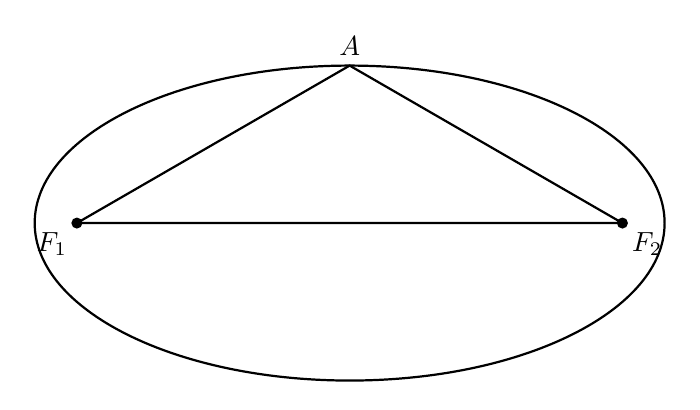
\begin{tikzpicture}
	
	% 定义椭圆的参数
	\def\a{4} % 半长轴长度 (a)
	\def\b{2} % 半短轴长度 (b)
	\pgfmathsetmacro{\c}{sqrt(\a*\a - \b*\b)} % 计算焦点到中心的距离 (c),使用公式 c = sqrt(a^2 - b^2)
	
	% 绘制椭圆
	\draw[thick] (0,0) ellipse (\a cm and \b cm); % 以 (0,0) 为中心,绘制半长轴为 a,半短轴为 b 的椭圆
	
	% 绘制焦点
	\fill (-\c,0) circle (2pt) node[below left] {$F_1$}; % 焦点 F1 位于 (-c, 0),用小圆点表示,并标注
	\fill (\c,0) circle (2pt) node[below right] {$F_2$}; % 焦点 F2 位于 (c, 0),用小圆点表示,并标注
	
	% 定义三角形的顶点坐标
	\coordinate (A) at (-\c, 0); % 焦点 F1 的坐标
	\coordinate (B) at (\c, 0); % 焦点 F2 的坐标
	\coordinate (C) at (0, \b); % 椭圆上的一个点 (0, b),在椭圆的顶点上
	
	% 绘制连接焦点和椭圆点的三角形
	\draw[thick] (A) -- (B) -- (C) -- cycle; % 连接 A, B, C,形成三角形
	
	% 标注三角形的点
	\node[above] at (C) {$A$}; % 在点 C (0, b) 位置标注 P
	
	% 可选:绘制从焦点到椭圆上的点的虚线
	\draw[dashed] (A) -- (C); % 从焦点 F1 到点 P 的虚线
	\draw[dashed] (B) -- (C); % 从焦点 F2 到点 P 的虚线
	
\end{tikzpicture}

\subsubsection{小焦点三角形}
	\[
\left.
\begin{aligned}
	|AF_{1}|+|AF_{2}|=2a \\
	|F_{1}F_{2}|=2c
\end{aligned}
\right\}
\Rightarrow C_{\vartriangle AF_{1}F_{2}}=2a+2c
\]
\subsubsection{大焦点三角形}

\[C_{\vartriangle ABF_{2}}=|AF_{1}|+|AF_{2}|+|BF_{1}|+|BF_{2}|=4a\]

\subsection{焦点弦}

\textit{过焦点的与相交的叫做焦点弦}
\[y=k(x\pm c)\]

%\begin{tcolorbox}[colback=white!10!white, colframe=yellow!50!black,title=eg]
	%$C=\dfrac{x^{2}}{2}+y^{2}=1$ \quad F为C的左焦点 P为C上一动点
	
	%Q(4,3)
	
%	(|PQ|+|PF|)_{MAX}
%\end{tcolorbox}
\[\star\ |PF_{1}|+|PF_{2}|=2a \Rightarrow |PF_{1}|=2a-|PF_{2}|\ \star\]
\subsection{焦点三角形面积}
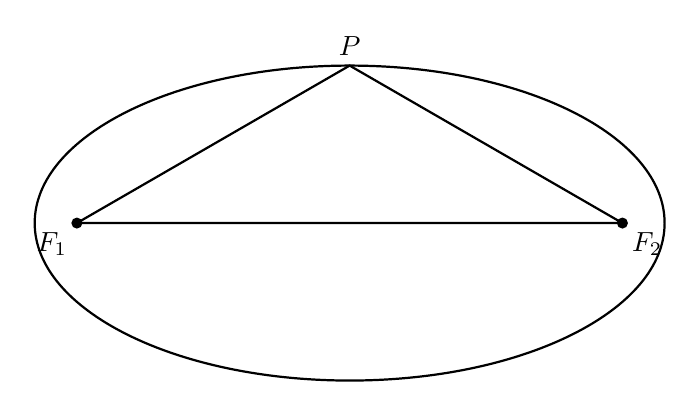
\begin{tikzpicture}
	
	% 定义椭圆的参数
	\def\a{4} % 半长轴长度 (a)
	\def\b{2} % 半短轴长度 (b)
	\pgfmathsetmacro{\c}{sqrt(\a*\a - \b*\b)} % 计算焦点到中心的距离 (c),使用公式 c = sqrt(a^2 - b^2)
	
	% 绘制椭圆
	\draw[thick] (0,0) ellipse (\a cm and \b cm); % 以 (0,0) 为中心,绘制半长轴为 a,半短轴为 b 的椭圆
	
	% 绘制焦点
	\fill (-\c,0) circle (2pt) node[below left] {$F_1$}; % 焦点 F1 位于 (-c, 0),用小圆点表示,并标注
	\fill (\c,0) circle (2pt) node[below right] {$F_2$}; % 焦点 F2 位于 (c, 0),用小圆点表示,并标注
	
	% 定义三角形的顶点坐标
	\coordinate (A) at (-\c, 0); % 焦点 F1 的坐标
	\coordinate (B) at (\c, 0); % 焦点 F2 的坐标
	\coordinate (C) at (0, \b); % 椭圆上的一个点 (0, b),在椭圆的顶点上
	
	% 绘制连接焦点和椭圆点的三角形
	\draw[thick] (A) -- (B) -- (C) -- cycle; % 连接 A, B, C,形成三角形
	
	% 标注三角形的点
	\node[above] at (C) {$P$}; % 在点 C (0, b) 位置标注 P
	
	% 可选:绘制从焦点到椭圆上的点的虚线
	\draw[dashed] (A) -- (C); % 从焦点 F1 到点 P 的虚线
	\draw[dashed] (B) -- (C); % 从焦点 F2 到点 P 的虚线
	
\end{tikzpicture}
\subsubsection{MAX}

当P点位于上/下顶点时,顶角$\angle F_{1}PF_{2}$取到最大值
\[\dfrac{1}{2}\cdotp 2\cdotp c \cdotp b =bc\]
\subsubsection{面积公式}
%\begin{tcolorbox}[colback=white!10!white, colframe=yellow!50!black]
%m+n=2a

%$ \cos \alpha =\dfrac{m^{2}+n^{2}-4c^{2}}{2mn} \Rightarrow mn=\dfrac{2b^{2}}{\cos \alpha +1}$

%$\cos 2\theta =2{\cos}^{2}\theta -1$
%$S=\dfrac{1}{2}\cdot \dfrac{2b^{2}\cdot sin \dfrac \theta}{cos \alpha +1}=b^{2} \cdot tan \dfrac{ \alpha }{2}$
%\end{tcolorbox}
\[b^2 \cdot \tan \left( \frac{\alpha}{2} \right)\]
	\[\mbox{双曲线}\dfrac{b^2}{\tan \left( \frac{\alpha}{2} \right)} \]
	\subsection{距离}
	\subsubsection{椭圆上的点到中心的距离|PO|}
	\[[a,b]\]
	\subsubsection{椭圆上的点到焦点的距离|PF|}
	\[[a-c,a+c]\]
	\subsection{椭圆的第二定义}
	
	动点到定点距离只比动点到定直线的距离只比为定值,则动点的轨迹为椭圆
	
	定点-焦点$(\pm c,0)$
	
	定直线-准线$x= \pm \dfrac{a^{2}}{c}$
	
	定值-$e=\dfrac{c}{a}$
	\[|PF|=a \pm ex_{0}\]
	\subsection{椭圆的参数方程}
		\[\dfrac{x^{2}}{a^{2}}+\dfrac{y^{2}}{b^{2}}=1 \Rightarrow
	\left\{
	\begin{aligned}
		x  = & a \cdot \cos(\theta) \\
		y  = & b \cdot \sin(\theta) \\
	\end{aligned}
	\right.
	\]
	\section{双曲线}
	
\begin{tikzpicture}
	
	% 定义双曲线参数
	\def\a{1} % 半实轴长度
	\def\b{1} % 半虚轴长度
	
	% 绘制双曲线
	\draw[samples=100, domain=-2:2, variable=\t]
	plot ({\a*cosh(\t)}, {\b*sinh(\t)}) % 右半部分
	plot ({-\a*cosh(\t)}, {\b*sinh(\t)}); % 左半部分
	
	% 绘制实轴和虚轴
	\draw[->] (-3,0) -- (3,0) node[right] {$x$}; % 实轴
	\draw[->] (0,-2) -- (0,2) node[above] {$y$}; % 虚轴
	
	% 标出渐近线
	\draw[dashed] (-3,-2) -- (3,2) node[right] {$y = \dfrac{b}{a}$}; % 正渐近线
	\draw[dashed] (-3,2) -- (3,-2) node[right] {$y = - \dfrac{b}{a}$}; % 负渐近线
	
	% 添加注释
	\node at (-2,-2) {双曲线};
	\node at (2.5,0.5) {实轴};
	\node at (0.5,1.5) {虚轴};
	
\end{tikzpicture}

\begin{longtable}{|c|c|}
	% 绘制表头的横线
	\hline
	% 定义表头内容
	双曲线 & $\dfrac{x^{2}}{a^{2}}-\dfrac{y^{2}}{b^{2}}=1$  \\
	% 绘制表头内容下的横线
	\hline
	% 指定 first head 的结束位置
	\endfirsthead
	
	% 绘制非第一页的表头的横线
	\hline
	% 定义非第一页的表头内容
	双曲线 & $\dfrac{x^{2}}{a^{2}}-\dfrac{y^{2}}{b^{2}}=1$  \\
	% 绘制表头内容下的横线
	\hline
	% 指定 head 的结束位置
	\endhead
	
	% 绘制每页底部的横线
	\hline
	% 指定 foot 的结束位置
	\endfoot
	
	% 绘制最后一页底部的横线
	\hline
	% 指定 last foot 的结束位置
	\endlastfoot
	
	% 表格主体部分
	范围 & $ x \in ( -\infty ,-a] \cup [a,+\infty) $ \\
	\hline
	顶点 &  (a,0),(-a,0)\\
	\hline
	焦点坐标 & $F_{1}(c,0) \quad F_{2}(-c,0)$  \\
	\hline
	abc关系 & $c^{2}=a^{2}+b^{2}$  \\
	\hline
	实轴 & 2a  \\
	\hline
	虚轴 & 2b    \\
	\hline
	焦距 & 2c   \\
	\hline
	$\star$离心率 & $e=\dfrac{a}{c} \in (1,+\infty)$ \\
	\hline
	通经 & $\dfrac{2b^{2}}{a}$   \\
	\hline
\end{longtable}

\end{document}